%
% Template Laporan Skripsi/Thesis 
%
% @author  Andreas Febrian, Lia Sadita 
% @version 1.03
%
% Dokumen ini dibuat berdasarkan standar IEEE dalam membuat class untuk 
% LaTeX dan konfigurasi LaTeX yang digunakan Fahrurrozi Rahman ketika 
% membuat laporan skripsi. Konfigurasi yang lama telah disesuaikan dengan 
% aturan penulisan thesis yang dikeluarkan UI pada tahun 2008.
%

%
% Tipe dokumen adalah report dengan satu kolom. 
%
\documentclass[12pt, a4paper, onecolumn, oneside, final]{report}

% Load konfigurasi LaTeX untuk tipe laporan thesis
\usepackage{style/uithesis}
\usepackage{natbib}
\usepackage{import}

% Load konfigurasi khusus untuk laporan yang sedang dibuat
%-----------------------------------------------------------------------------%
% Informasi Mengenai Dokumen
%-----------------------------------------------------------------------------%
% 
% Judul laporan. 
\var{\judul}{Desain dan Analisa Penerapan Pola Model-View-Controller (MVC)
    Untuk Pengembangan Software Product Line (SPL) Berbasis Web dengan
    Menggunakan Bahasa Pemodelan Abstract Behavioural Spesification (ABS)}
% 
% Tulis kembali judul laporan, kali ini akan diubah menjadi huruf kapital
\Var{\Judul}{Desain dan Analisa Penerapan Pola Model-View-Controller (MVC)
    Untuk Pengembangan Software Product Line (SPL) Berbasis Web dengan
    Menggunakan Bahasa Pemodelan Abstract Behavioural Spesification (ABS)}
% 
% Tulis kembali judul laporan namun dengan bahasa Ingris
\var{\judulInggris}{Analysis and Design of the Use of Model-View-Controller (MVC)
    Design Pattern for Web Based Software Product Line Engineering (SPLE) Using 
    Abstract Behavioural Specification (ABS) Modeling Language}

% 
% Tipe laporan, dapat berisi Skripsi, Tugas Akhir, Thesis, atau Disertasi
\var{\type}{Thesis}
% 
% Tulis kembali tipe laporan, kali ini akan diubah menjadi huruf kapital
\Var{\Type}{Thesis}
% 
% Tulis nama penulis 
\var{\penulis}{Salman El Farisi}
% 
% Tulis kembali nama penulis, kali ini akan diubah menjadi huruf kapital
\Var{\Penulis}{Salman El Farisi}
% 
% Tulis NPM penulis
\var{\npm}{1306346720}
% 
% Tuliskan Fakultas dimana penulis berada
\Var{\Fakultas}{Ilmu Komputer}
\var{\fakultas}{Ilmu Komputer}
% 
% Tuliskan Program Studi yang diambil penulis
\Var{\Program}{Magister Ilmu Komputer}
\var{\program}{Magister Ilmu Komputer}
\var{\programEng}{Master of Computer Science}
% 
% Tuliskan tahun publikasi laporan
\Var{\bulanTahun}{Desember 2014}
% 
% Tuliskan gelar yang akan diperoleh dengan menyerahkan laporan ini
\var{\gelar}{Magister Ilmu Komputer}
% 
% Tuliskan tanggal pengesahan laporan, waktu dimana laporan diserahkan ke 
% penguji/sekretariat
\var{\tanggalPengesahan}{21 Desember 2013} 
% 
% Tuliskan tanggal keputusan sidang dikeluarkan dan penulis dinyatakan 
% lulus/tidak lulus
\var{\tanggalLulus}{21 Desember 2013}
% 
% Tuliskan pembimbing 
\var{\pembimbing}{Dr. Ade Azurat}

% 
% Alias untuk memudahkan alur penulisan paa saat menulis laporan
\var{\saya}{Penulis}

% Daftar pemenggalan suku kata dan istilah dalam LaTeX
%
% Hyphenation untuk Indonesia 
%
% @author  Andreas Febrian
% @version 1.00
% 
% Tambahkan cara pemenggalan kata-kata yang salah dipenggal secara otomatis 
% oleh LaTeX. Jika kata tersebut dapat dipenggal dengan benar, maka tidak 
% perlu ditambahkan dalam berkas ini. Tanda pemenggalan kata menggunakan 
% tanda '-'; contoh:
% menarik
%   --> pemenggalan: me-na-rik
%

\hyphenation{
    % alphabhet A
    a-na-li-sa a-tur 
    a-pli-ka-si 
    % alphabhet B
    ba-ngun-an 
    be-be-ra-pa 
    ber-ge-rak
    ber-ke-lan-jut-an 
    ber-pe-nga-ruh 
    % alphabhet C
    ca-ri
    % alphabhet D
    di-ban-ding-kan
    di-de-fi-ni-si-kan
    di-ha-rap-kan
    di-ka-te-go-ri-kan
    di-mi-li-ki-nya
    di-se-rah-kan
    di-sim-pan di-pim-pin de-ngan da-e-rah di-ba-ngun da-pat di-nya-ta-kan 
    di-sim-bol-kan di-pi-lih di-li-hat de-fi-ni-si
    di-se-su-ai-kan
    % alphabhet E
    e-le-men
    e-ner-gi eks-klu-sif
    % alphabhet F
    fa-si-li-tas
    % alphabhet G
    ga-bung-an ge-rak
    % alphabhet H
    ha-lang-an
    he-te-ro-gen
    % alphabhet I
    i-ngin
    % alphabhet J
    % alphabhet K
    ke-hi-lang-an
    ku-ning 
    kua-li-tas ka-me-ra ke-mung-kin-an ke-se-pa-ham-an
    ke-te-pat-an
    kon-fi-gu-ra-si
    % alphabhet L
    ling-kung-an
    % alphabhet M
    me-min-ta
    me-mo-del-kan
    me-mo-ri
    men-de-fi-ni-si-kan
    me-neng-ah
    me-ne-ri-ma
    meng-a-tas-i me-mung-kin-kan me-nge-na-i me-ngi-rim-kan 
    meng-u-bah meng-a-dap-ta-si me-nya-ta-kan mo-di-fi-ka-si
    meng-a-tur
    meng-au-to-ma-si
    meng-a-ko-mo-da-si
    me-ngo-rek-si
    me-re-a-li-sa-si-kan
    % alphabhet N
    nya-ta non-eks-klu-sif
    % alphabhet O
    % alphabhet P
    pa-ra-lel
    peng-ala-mat-an
    pen-ting
    penga-da-an
	pe-nye-rap-an 
	pe-ngon-trol
    pe-mo-del-an
    pe-ran  pe-ran-an-nya
    pe-rin-tah
    pem-ba-ngun-an pre-si-den pe-me-rin-tah prio-ri-tas peng-am-bil-an 
    peng-ga-bung-an pe-nga-was-an pe-ngem-bang-an 
    pe-nga-ruh pa-ra-lel-is-me per-hi-tung-an per-ma-sa-lah-an 
    pen-ca-ri-an peng-struk-tur-an
    pe-ner-bang-an
    po-pu-ler
    pro-se-sor
    % alphabhet Q
    % alphabhet R
    ran-cang-an
    % alphabhet S
    se-dang-kan
    se-ring
    si-mu-la-si sa-ngat    
    % alphabhet T
    te-ngah
    ter-da-pat
    % alphabhet U
    u-sa-ha
    % alphabhet V
    % alphabhet W
    % alphabhet X
    % alphabhet Y
    % alphabhet Z
    % special
}
% Daftar istilah yang mungkin perlu ditandai 
%
% @author  Andreas Febrian
% @version 1.00
% 
% Mendaftar seluruh istilah yang mungkin akan perlu dijadikan 
% italic atau bold pada setiap kemunculannya dalam dokumen. 
% 

\var{\license}{\f{Creative Common License 1.0 Generic}}
\var{\bslash}{$\setminus$}


%\usepackage[backend=bibtex]{biblatex}
%\addbibresource{bib.bib}

% Awal bagian penulisan laporan
\begin{document}

%
% Sampul Laporan
%
% @author  unknown
% @version 1.01
% @edit by Andreas Febrian
%

\begin{titlepage}
    \begin{center}    
        \begin{figure}
            \begin{center}
                
\includegraphics[width=2.5cm]{img/makara.png}
            \end{center}
        \end{figure}    
        \vspace*{0cm}
        \bo{
        	UNIVERSITAS INDONESIA\\
        }
        
        \vspace*{1.0cm}
        % judul thesis harus dalam 14pt Times New Roman
        \bo{\Judul} \\[1.0cm]

        \vspace*{2.5 cm}    
        % harus dalam 14pt Times New Roman
        \bo{\Type}

        \vspace*{3 cm}       
        % penulis dan npm
        \bo{\Penulis} \\
        \bo{\npm} \\

        \vspace*{5.0cm}

        % informasi mengenai fakultas dan program studi
        \bo{
        	FAKULTAS \Fakultas\\
        	PROGRAM STUDI \Program \\
        	DEPOK \\
        	\bulanTahun
        }
    \end{center}
\end{titlepage}

\pagenumbering{roman}
\setcounter{page}{2}

\singlespacing
%
% Halaman Abstrak
%
% @author  Andreas Febrian
% @version 1.00
%

\chapter*{Abstrak}

\vspace*{0.2cm}

\noindent \begin{tabular}{l l p{10cm}}
	Nama&: & \penulis \\
	Program Studi&: & \program \\
	Judul&: & \judul \\
\end{tabular} \\ 

\vspace*{0.5cm}

\vspace*{0.2cm}

\noindent Kata Kunci: \\ 
\noindent \textit{Model-View-Controller} (MVC), \textit{Software Product Line} (SPL), \textit{Abstract Behavioural Specification} (ABS), \textit{Web Application}\\ 

\newpage
\tableofcontents
\clearpage
\listoffigures
\clearpage

\pagenumbering{arabic}
\onehalfspacing
\setlength{\parindent}{0pt}
\chapter{Pendahuluan}

%---------------------------------------------------------
\section{Latar Belakang}
%---------------------------------------------------------
Dalam perancangan produk perangkat lunak, tentunya kita akan mempertimbangkan tentang siapa yang akan menggunakan perangkat lunak tersebut. Hal ini tetunya harus dilakukan karena kita menginginkan bahwa perangkat lunak yang dibuat memiliki fungsionalitas yang sesuai dengan kebutuhan para penggunanya. Oleh karena itu, dalam sebuah perancangan perangkat lunak diperlukan adanya proses pengumpulan informasi kebutuhan (\textit{requirement gathering}) agar rancangan perangkat lunak yang kita buat sesuai dengan ekspektasi dan kebutuhan pengguna. \\

\noindent
Berbicara tentang \textit{requirement} perangkat lunak, kita mengetahui bahwa seiring berjalannya waktu, jumlah dan tingkat kompleksitas dari \textit{requirement} sebuah perangkat lunak akan semakin meningkat. Hal ini tentunya disebabkan oleh semakin tingginya kebutuhan dan luasnya domain permasalahan para pengguna yang harus ditangani oleh perangkat lunak tersebut. Dampak dari dua hal tersebut pada akhirnya memaksa para pengembang perangkat lunak untuk terus melakukan perubahan (evolusi) terhadap perangkat lunak yang dibuatnya. Apabila proses evolusi perangkat lunak tersebut tidak sebanding dengan peningkatan kebutuhan pengguna, maka para pengguna perangkat lunak tersebut akan berpaling ke perangkat lunak lain yang dinilai dapat memenuhi kebutuhan mereka saat ini. \\

\noindent
Salah satu pendekatan yang dapat digunakan untuk melakukan proses evolusi produk perangkat lunak secara cepat dan efisien adalah dengan menggunakan pendekatan \textit{Software Product Line Engineering} (SPLE). SPLE merupakan sebuah paradigma yang digunakan dalam proses pengembangan perangkat lunak dengan menggunakan konsep \textit{software platform} dan \textit{mass customisation} \citep[p.~14]{pohl2005software}. Dengan menggunakan paradigma ini, proses evolusi produk perangkat lunak dapat dilakukan dengan melihat aspek \textit{commonality} dan \textit{variability} dari komponen-komponen yang ada. Hal ini tentunya akan membuat proses evolusi produk perangkat lunak menjadi lebih cepat dan efisien dikarenakan para pengembang produk perangkat lunak tidak perlu mengembangkan produknya dari awal untuk memenuhi variasi dari kebutuhan yang sama. \\

\noindent
Salah satu teknologi yang dapat digunakan dalam melakukan pengembangan \textit{Software Product Line} (SPL) adalah \textit{Abstract Behavioural Spesification} (ABS). ABS adalah sebuah bahasa pemodelan yang dibuat oleh konsorsium uni eropa sejak tahun 2008 dengan nama proyek \textit{Highly Adaptable and Trustworthy Software using Formal Methods} (HATS). bahasa pemodelan ini didesain khusus memiliki kemampuan untuk melakukan pemodelan fitur dan delta sehingga dapat digunakan untuk membuat SPL. Secara sintaksis, ABS memiliki sintaks yang mirip dengan bahasa pemrograman JAVA. Kemiripan sintaks ABS dengan JAVA sengaja dibuat agar para pengembang perangkat lunak dengan mudah beradaptasi dengan bahasa pemodelan ini \citep{hahnle2013hats}. \\

\noindent
Dalam proses pengembangan perangkat lunak, \textit{code reuse} dan \textit{code maintenance} menjadi hal yang harus diperhatikan dengan baik. Kedua aspek tersebut mendapat perhatian khusus dikarenakan proyek perangkat lunak merupakan proyek yang berkepanjangan (terus berevolusi) dan memerlukan tingkat kolaborasi yang tinggi (terutama untuk perangkat lunak dengan sekala yang besar). Salah satu \textit{best practice} yang digunakan untuk dapat mewujudkan kedua aspek tersebut adalah dengan menggunakan sebuah pendekatan yang bernama \textit{Model-View-Controller} (MVC). MVC merupakan sebuah pendekatan yang digunakan dalam proses perangkat lunak untuk memisahkan antara logika aplikasi, data, dan presentasi \citep{leff2001web} \citep{krasner1988desc}. Dalam penelitian ini, penulis akan membuat sebuah \textit{framework} MVC untuk ABS yang nantinya akan digunakan dalam proses pengembangan SPL berbasis web.

%---------------------------------------------------------
\section{Manfaat Penelitian}
%---------------------------------------------------------
Adapun manfaat dari penelitian yang dilakukan antara lain adalah:
\begin{enumerate}
    \item Memberikan pengetahuan lebih lanjut terkait bagaimana melakukan perancangan dan penerapan pola \textit{Model-View-Controller} dalam melakukan pengembangan SPL berbasis web dengan menggunakan bahasa pemodelan ABS.
    \item Membuktikan bahwa bahasa pemodelan ABS juga dapat digunakan dalam pengembangan aplikasi \textit{frontend} dan bukan hanya untuk aplikasi \textit{backend} yang tidak memiliki \textit{user interface} (seperti yang dilakukan selama ini).
    \item Menghasilkan sebuah \textit{framework} MVC ABS yang dapat digunakan oleh para pengembang perangkat lunak untuk dapat membuat SPL berbasis web dengan menggunakan ABS.
\end{enumerate}

%---------------------------------------------------------
\section{Kerangka Berpikir}
%---------------------------------------------------------
\noindent
Tujuan utama dari dilakukannya penelitian ini adalah adalah untuk menganalisa dan merancang strategi pengembangan SPL berbasis web dengan menggunakan bahasa pemodelan ABS. Ketika berbicara tentang perangkat lunak berbasis web, tentunya kita juga harus memikirkan bagaimana caranya agar perangkat lunak yang sudah dibuat dapat berjalan di \textit{web server}. Dalam konteks ABS, penulis perlu mencari tahu bagaimana caranya agar ABS dapat berjalan di atas platform JAVA \textit{Application Server} yang sudah ada seperti misalnya Apache Tomcat atau Oracle Glassfish. Apabila ABS tidak dapat dijalankan di atas platform yang sudah ada, maka penulis harus membuat sendiri sebuah \textit{Application Server} yang dapat menjalankan ABS.

\begin{figure}
    \centering
    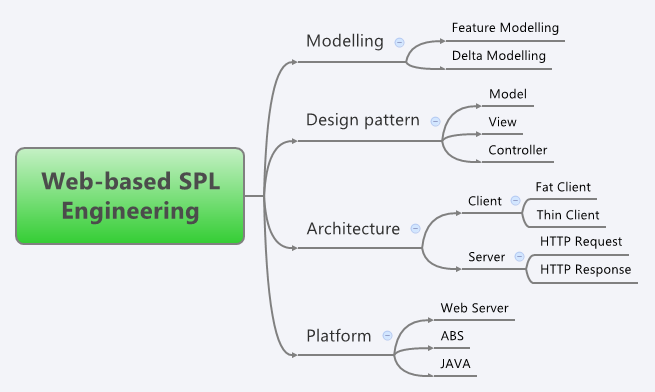
\includegraphics[width=0.8\textwidth]
        {img/kerangka-berpikir.png}
    \caption{Kerangka berpikir}
\end{figure}

\noindent
Setelah penulis mengetahui solusi apa yang harus digunakan agar ABS dapat berjalan di \textit{Application Server}, selanjutnya penulis akan merancang bagaimana pengorganisasian kode yang baik untuk ABS agar sesuai dengan kaidah MVC. Hal ini perlu dilakukan karena nantinya penelitian ini akan menghasilkan sebuah \textit{framework} MVC yang akan digunakan dalam pengembangan SPL berbasis web dengan menggunakan ABS. Dalam hal ini, penulis harus mengkaji terkait peran-peran setiap komponen pada MVC dan kemudian mengimplementasikannya ke ABS. \\

\noindent
Rangkaian proses diatas diharapkan nantinya menghasilkan sebuah framwork MVC yang utuh untuk kemudian diintegrasikan dengan konsep \textit{feature modelling} dan \textit{delta modelling} yang ada di ABS. Hal ini dilakukan agar dapat dihasilkan sebuah framework MVC ABS yang dapat digunakan untuk keperluan pengembangan SPL berbasis web.

%---------------------------------------------------------
\section{Sistematika Penulisan}
%---------------------------------------------------------
berikut adalah sistematika penulisan dari proposal ini:
\begin{itemize}
    \item Bab 1 Pendahuluan \\
    Bab ini berisi tentang latar belakang penelitian, manfaat penelitian, kerangka berpikir, dan sistematika penulisan.
    \item Bab 2 Studi Literatur \\
    Bab ini berisi tentang hasil studi literatur yang dilakukan oleh penulis baik terkait teori-teori dasar yang mendukung penelitian ini ataupun peneletian lain yang masih berkaitan dengan penelitian yang akan dilakukan.
    \item Bab 3 Rumusan Masalah \\
    Bab ini berisi tentang rumusan masalah dari penelitian yang akan dilakukan, ruang lingkup penelitian, serta batasan penelitian.
    \item Bab 4 Rancangan Penelitian \\
    Bab ini berisi tentang rancangan penelitian yang akan dilakukan oleh penulis dan penjelasan dari setiap tahapan-tahapan yang akan dilakukan.
\end{itemize}
\include{RumusanMasalah}
\chapter{Hasil Studi Literatur}

%---------------------------------------------------------
\section{Model View Controller}
%---------------------------------------------------------
\noindent
\textit{Model-View-Controller} (MVC) atau yang biasa juga dikenal dengan sebutan \textit{Presentation-Abstraction-Control} (PAC) merupakan salah satu pendekatan dalam proses pengembangan perangkat lunak yang ditujukan untuk melakukan pemisahan antara logika aplikasi, data, dan presentasi. Konsep ini dibangun atas kesadaran bahwa sebuah model domain aplikasi yang sama dapat disajikan dan diperlakukan secara berbeda tergantung dari kebutuhan si pengguna aplikasi. Dengan menggunakan pendekatan ini, seorang pengembang perangkat lunak dapat berfokus pada satu bagian saja tanpa harus mengkhawatirkan akan terkena dampak perubahan ataupun memberikan perubahan ke bagian aplikasi lainnya.

\subsection{Sejarah Singkat MVC}
\noindent
Konsep MVC diterapkan pertama kalinya oleh Alan Kay, Dan Ingalls, dan Adele Goldberg pada tahun 1980 ketika mereka merancang bahasa pemrograman smalltalk-80 di Xerox PARC Learning Research Group (LRG) \citep{krasner1988desc}. bahasa pemrograman ini didesain dan dikembangkan dengan menggunakan strategi yang merepresentasikan informasi, tampilan, dan kontrol pada lingkungan pemrogramannya. Strategi ini digunakan dengan tujuan (1) untuk membuat kumpulan komponen sistem spesial yang dibutuhkan dalam mendukung proses pengembangan perangkat lunak yang interaktif serta (2) menyediakan kumpulan komponen sistem umum yang dapat membantu pengembang dalam menciptakan aplikasi grafis yang interaktif dengan mudah \citep{krasner1988desc}. Strategi dan tujuan tersebut dibuat dalam rangka menjawab isu utama dalam pengembangan perangkat lunak yaitu terkait pemanfaatan kembali komponen yang telah dibuat (\textit{reusability}) dan kemudahan dalam menggabungkan setiap komponen aplikasi (\textit{plugability}). \\

\noindent
Belajar dari pengalamannya dalam mengembangkan smalltalk-76, para pengembang smalltalk-80 menemukan bahwa untuk mencapai sebuah modularitas yang tinggi diperlukan adanya tiga buah pemisahan fokus dalam pengembangan aplikasi. Tiga buah pemisahan fokus tersebut antara lain adalah (1) memisahkan setiap komponen yang merepresentasikan model domain aplikasi dengan (2) cara yang digunakan untuk merepresentasikan model tersebut ke pengguna aplikasi dan (3) cara yang digunakan oleh pengguna dalam berinteraksi dengan model tersebut. Tiga buah pemisahan tersebut dapat terangkum dalam sebuah konsep yang disebut dengan \textit{Model-View-Controller} (MVC).

\subsection{Penerapan MVC dalam Pengembangan Aplikasi Web}
Aplikasi web merupakan aplikasi yang tergolong interaktif karena aplikasi jenis ini banyak memiliki elemen-elemen yang dapat digunakan untuk berinteraksi dengan penggunannya. Sebagai contoh, dalam sebuah halaman situs web tentunya kita akan menemukan banyak tombol, gambar, tautan, dan kotak isian yang dapat kita gunakan untuk berinteraksi dengan situs web tersebut. Untuk sebuah aplikasi yang tergolong interaktif, adanya pemisahan antara logika aplikasi, data, dan presentasi tentunya akan dapat meningkatkan fleksibilitas aplikasi tersebut dari segi pengembangan. \\

\noindent
Pada dasarnya, arsitektur apliksi berbasis web terbagi menjadi dua bagian yaitu \textit{client} dan \textit{server}. Dengan arsitektur yang seperti ini, para pengembang aplikasi tidak dapat menentukan dengan jelas bagaimana bentuk partisi yang harus dibuat untuk aplikasi tersebut. Sebagai contoh, dengan adanya pembagian antara \textit{client} dan \textit{server}, para pengembang aplikasi harus menentukan dimanakah komponen \textit{view} akan dibentuk? Apakah komponen ini akan dibentuk di tingkat \textit{client} ataukah di tingkat \textit{server}. Begitupun dengan komponen \textit{Model} dan \textit{Controller
}-nya. Apakah komponen-komponen tersebut akan akan dibuat di tingkat \textit{client}, \textit{server}, atau keduanya? Pada akhirnya, keputusan dalam menentukan skema partisi yang dipakai akan sangat bergantung pada teknologi yang digunakan \citep{leff2001web}. \\

\noindent
Permasalahan terkait pemisahan antara \textit{client} dan \textit{server} pada aplikasi berbasis web menjadikan penerapan MVC lebih sulit. Proses penerapan MVC akan dapat berhasil apabila (1) para pengembang aplikasi sudah mengetahui bagaimana skema partisi yang akan diterapkan serta (2) teknologi dan infrastruktur yang ada \textit{compatible} dengan skema partisi yang diterapkan. Oleh karena itu, perlu adanya sebuah pendekatan yang dapat digunakan oleh para pengembang untuk memastikan dua hal tersebut.

%---------------------------------------------------------
\section{Software Product Line Engineering (SPLE)}
%---------------------------------------------------------
\noindent
\textit{Software Product Line Engineering} (SPLE) merupakan sebuah paradigma yang digunakan dalam proses pengembangan perangkat lunak dengan menggunakan prinsip \textit{platform} dan \textit{mass customisation} \citep[p.~14]{pohl2005software}. Dalam industri perangkat lunak, istilah \textit{platform} atau \textit{software platform} biasa diartikan sebagai sebuah sistem komputer (misal: prosesor atau kombinasi antara perangkat keras dengan sistem operasi) yang menyebabkan dapat berjalannya sebuah program komputer. Sedangkan dalam konteks SPLE, yang dimaksud dengan \textit{platform} adalah sebuah subsistem dan \textit{interface} yang membentuk sebuah struktur umum dimana nantinya sebuah produk turunan dapat dikembangkan dan diproduksi secara efisien \citep[p.~15]{pohl2005software}. \\

\noindent
Dalam paradigma SPLE, proses pengembangan perangkat lunak dibagi menjadi dua bagian yaitu \textit{Domain Engineering} dan \textit{Application Engineering} \citep[p.~21]{pohl2005software}. \textit{Domain Engineering} adalah sebuah proses dalam SPLE dimana pada tahap ini seluruh \textit{commonality} dan \textit{variability} dari SPL didefinisikan dan direalisikan. Sedangkan tahap \textit{Application Engineering} adalah sebuah proses dimana aplikasi dari SPL dibuat dengan cara memanfaatkan \textit{domain artifact} yang telah dibuat pada tahap sebelumnya dan mengeksploitasi \textit{variability} yang ada di dalam SPL tersebut. Tahapan-tahapan proses dalam SPLE ini biasa disebut dengan istilah \textit{SPLE Framework}. \\

\begin{figure}
    \centering
    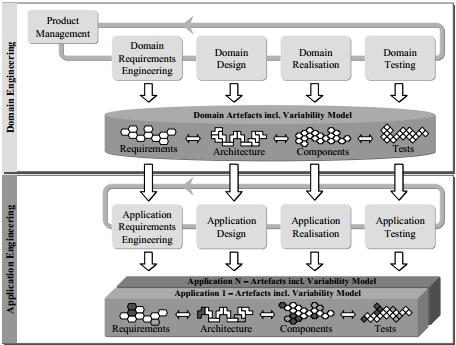
\includegraphics[width=0.8\textwidth]
        {img/sple-process.png}
    \caption{SPLE Framework}
\end{figure}
\vspace{-0.8cm}
\begin{center}
{\small Sumber gambar: \citep{pohl2005software}}
\end{center}

%---------------------------------------------------------
\section{Abstract Behavioural Spesification (ABS)}
%---------------------------------------------------------
\noindent
Abstract Behavioural Specification Language (ABS) merupakan sebuah bahasa pemodelan yang dibuat oleh konsorsium uni eropa di bawah proyek bernama \textit{Highly Adaptable and Trustworthy Software using Formal Method} (HATS). Tujuan dari proyek HATS dalam menciptakan ABS adalah untuk menciptakan sebuah pendekatan yang \textit{model-centric} dalam melakukan proses perancangan, implementasi dan verifikasi dari sebuah sistem yang \textit{highly-configurable} \citep{clarke2012variability}. Pada dasarnya ABS dibagi kedalam beberapa layer (lihat gambar 2.x) yang diantaranya adalah \textit{functional abstraction}, \textit{OO-Imperative layer}, \textit{Concurency Model} dan \textit{ABS Core}. \\

\begin{figure}
    \centering
    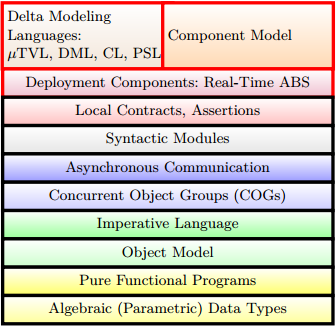
\includegraphics[width=0.6\textwidth]
        {img/abs-layers.png}
    \caption{ABS Layer}
\end{figure}
\vspace{-0.8cm}
\begin{center}
{\small Sumber gambar: \citep{hahnle2013hats}}
\end{center}

\noindent
Sebagai sebuah bahasa pemrograman \textit{imperative} yang menganut konsep \textit{Object Oriented}, secara umum ABS memiliki sintaks yang sama dengan bahasa pemrograman JAVA (walaupun lebih sederhana). Salah satu perbedaan yang paling mendasar antara ABS dengan JAVA adalah pada konsep \textit{code reuse}-nya. Pada bahasa pemrograman JAVA, konsep \textit{code reuse} diimplementasikan dengan cara membuat \textit{code inheritance} sedangkan pada ABS konsep tersebut diimplementasikan dalam betuk \textit{code deltas} \citep{hahnle2013hats}. \textit{code deltas} pada ABS merupakan sebuah kumpulan kode yang mendeskripsikan perubahan-perubahan kode pada kelas yang dituju. Dengan adanya konsep ini, ABS dapat melakukan manipulasi kelas seperti menambah atau menghilangkan \textit{variable} dan \textit{method}. \\

\noindent
Seperti yang sudah disebutkan sebelumnya bahwa di dalam ABS konsep \textit{code reuse} diimplementasikan dalam bentuk \textit{code deltas}. \textit{Code deltas} tersebut nantinya akan digunakan untuk memodelkan \textit{variability} yang terjadi di tingkat \textit{source code}. pemodelan \textit{variability} ini merupakan sebuah pendekatan yang dilakukan oleh ABS dalam membangun sebuah SPL. Proses pemodelan \textit{variability} ini biasa disebut juga sebagai proses \textit{Delta Modelling}. \\

\noindent
\textit{Delta Modelling} merupakan sebuah pendekatan yang fleksible dan modular dalam mewujudkan berbagai macam variasi produk dengan menggunakan kembali artifak-artifak yang ada \citep{hahnle2013hats}. Dalam proses \textit{Delta Modelling}, realisasi dari SPL dibentuk dari dua bagian yaitu \textit{core module} dan \textit{delta module}. \textit{Delta module} berisi fungsi-fungsi yang berlaku umum terhadap semua varian produk yang akan dibuat sedangkan \textit{delta modul} merupakan enkapsulasi dari perubahan-perubahan yang akan terjadi pada \textit{core product} untuk kemudian menghasilkan varian produk yang lain. \\

\begin{figure}
    \centering
    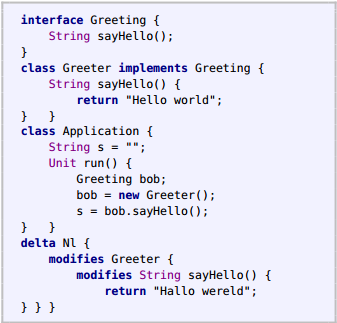
\includegraphics[width=0.6\textwidth]
        {img/delta-modelling-1.png}
\end{figure}

\begin{figure}
    \centering
    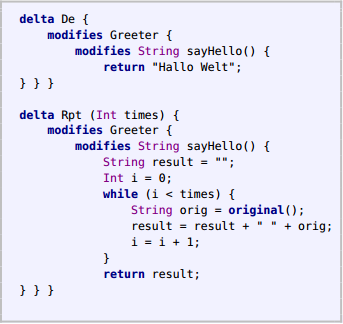
\includegraphics[width=0.6\textwidth]
        {img/delta-modelling-2.png}
    \caption{Delta Modelling pada ABS}
\end{figure}\vspace{-0.8cm}
\begin{center}
{\small Sumber gambar: \citep{clarke2012variability}}
\end{center}
\chapter{Metodologi Penelitian}

Berdasarkan rumusan masalah, ruang lingkup penelitian, serta batasan penelitian yang sudah dibahas pada bab sebelumnya, berikut ini adalah metodologi penelitian yang penulis gunakan:

\begin{figure}
    \centering
    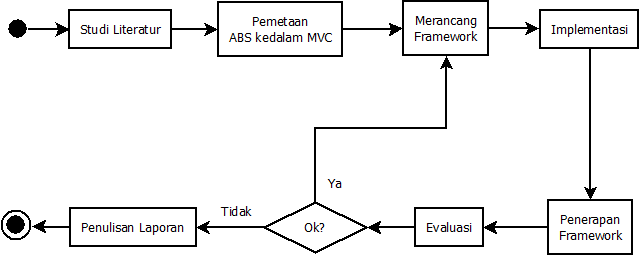
\includegraphics[width=0.8\textwidth]
        {img/metodologi-penelitian.png}
    \caption{Rencana Penelitian}
    \label{fig:metodologiPenelitian}
\end{figure}

Seperti yang terlihat pada Gambar \ref{fig:metodologiPenelitian} diatas, pada awal penelitian penulis melakukan studi literatur untuk mendapatkan pengetahuan terkait teori-teori pendukung yang penulis gunakan dalam melakukan penelitian. Setelah selesai melakukan studi literatur, berikutnya penulis melakukan proses analisa dan pemetaan terhadap bahasa pemodelan ABS untuk kemudian dilakukan pemetaan kedalam komponen-komponen MVC. Seteah proses pemetaan selesai, penulis membuat rancangan ABS MVC Framework sesuai dengan hasil analisa dan pemetaan yang telah dilakukan dan setelah itu penulis melakukan proses implementasi untuk merealisasikan desain yang telah dibuat. Langkah berikutnya adalah melakukan proses penerapan ABS MVC Framework untuk melihat apakah \textit{framework} yang dibuat dapat digunakan untuk membuat sebuah aplikasi berbasis web dan melakukan evaluasi terhadap \textit{framework} tersebut untuk menentukan apakah harus dilakukan perombakan atau sudah layak sebagai sebuah MVC Framework. Berikut ini adalah detail dari setiap tahapan penelitian yang penulis lakukan:

\section{Studi Literatur}

Pada tahap ini penulis melakukan studi literatur dari berbagai sumber seperti buku, artikel ilmian dan web untuk mendapatkan informasi dan pengetahuan terkait teori pendukung yang penulis butuhkan dalam melakukan penelitian ini. Adapun pengetahuan-pengetahuan pendukung yang penulis butuhkan antara lain adalah pengetahuan tentang Hypertext Transfer Protocol (HTTP), pola Model-View-Controller (MVC) dalam pengembangan perangkat lunak, pengetahuan tentang bahasa pemodelan ABS dan pengetahuan tentang \textit{Software Product Line Engineering} (SPLE).

\section{Pemetaan ABS kedalam MVC}

Pada tahap ini penulis melakukan analisa terhadap bahasa pemodelan ABS sesuai dengan pengetahuan yang penulis dapatkan dalam proses studi literatur yang sudah penulis lakukan sebelumnya. Tujuan dari proses analisa yang penulis lakukan ini adalah untuk memetakan bahasa pemodelan ABS kedalam komponen-komponen ABS.

\section{Merancang ABS MVC Framework}

Pada tahap ini penulis membuat rancangan ABS MVC Framework berdasarkan hasil analisa dan pemetaan ABS yang dibuat sebelumnya. Adapun rancangan yang dibuat adalah mengenai bagaimana penyusunan direktori dari \textit{framework} tersebut, bagaiamana karakteristik dari setiap komponen MVC yang dibuat dengan menggunakan ABS serta bagaimana caranya agar komponen MVC yang dibuat dapat menghasilkan sebuah halaman web.

\section{Implementasi}

Pada tahap ini penulis merealisasikan rancangan ABS MVC Framework yang telah penulis buat sebelumnya. Adapun poin-poin implementasi yang dilakukan antara lain adalah mengintegrasikan \textit{framework} ABS yang dibuat dengan JAVA dan \textit{web server} agar \textit{framework} tersebut dapat menghasilkan sebuah halaman web yang utuh.

\section{Penerapan ABS MVC Framework}

Pada tahap ini penulis membuat sebuah aplikasi web dengan menggunakan ABS MVC Framework yang dibuat sekaligus mencoba untuk menerapkan \textit{delta modeling} dan SPLE terhadap \textit{framework} tersebut.

\section{Evaluasi}

Pada tahap ini penulis mengevaluasi hasil penerapan yang dilakukan untuk melihat apakah pelu adanya revisi dan perancangan ulang atau \textit{framework} tersebut sudah sesuai dengan tujuan dari penelitian ini. Apabila hasil evaluasi dari \textit{framework} yang dibuat belum memuaskan, makan akan dilakukan proses revisi rancangan untuk lebih menyempurnakan lagi \textit{framework} yang dibuat. Namun, apabila hasil evaluasi sudah memuaskan maka langkah selanjutnya adalah mendokumentasikan hasil penelitian yang diperoleh kadalam laporan penelitian. Adapun syarat-syarat kelayakan yang penulis tetapkan sebagai parameter keberhasilan dalam proses evaluasi ini antara lain adalah:

\begin{enumerate}
    \item Apakah \textit{framework} yang dihasilkan sudah sesuai dengan kaidah MVC yang berlaku? (sesuai dengan yang ada pada studi literatur)
    \item Apakah \textit{framework} yan dihasilkan dapat diintegrasikan dengan \textit{feature modeling} dan \textit{delta modeling} pada ABS?
    \item Apakah \textit{framework} yang dihasilkan sudah dapat mengasilkan sebuah \textit{complete product} SPL berbasis web? (dapat dijalankan)
\end{enumerate}

\section{Penulisan Laporan}

Pada tahap ini penulis akan menuliskan laporan penelitian dan menarik kesimpulan yang diambil dari penelitian yang sudah dilakukan serta memaparkan temuan-temuan yang diperoleh selama melakukan penelitian.
\chapter{Eksperimen}
Bab ini memaparkan secara kronologis tentang proses eksperimen yang telah dilakukan oleh penulis.

\section{Mengintegrasikan ABS dengan JAVA}
Berdasarkan hasil studi literatur yang telah dilakukan, penulis mengetahui bahwa salah satu fitur yang dimiliki oleh ABS adalah kemampuannya untuk dapat di\textit{compile} kedalam bahasa JAVA sehingga nantinya kode ABS tersebut dapat dijalankan di dalam JAVA Runtime Environment (JRE). Berdasarkan informasi tersebut, penulis menarik kesimpulan bahwa jika penulis membuat sebuah JAVA class yang dibuat secara \textit{native}, maka JAVA Class tersebut akan dapat memanggil class ABS yang sudah di\textit{compile} menjadi JAVA Class juga.\\

Sebelum penulis mencoba untuk mengintegrasikan secara langsung ABS dengan JAVA, penulis mencoba untuk mengetahui hasil kompilasi kode ABS yang diubah kedalam JAVA. berikut adalah kode ABS sederhana yang penulis buat beserta hasil kompilasinya ke dalam kode JAVA.

\begin{lstlisting}[
caption=Kode ABS beserta Main Blocknya,
label={lst:absSederhana},
escapeinside={@}{@}
]
module UserModule;

interface User
{
	String getUsername();
}

class UserImpl implements User
{
	String getUsername() @\label{lst:absString}@
	{
		return "salman"; @\label{lst:absString2}@
	}
}

//ABS Main block
{
	User myUser = new local UserImpl(); @\label{lst:absCreateObject}@
	String username = myUser.getUsername();
}
\end{lstlisting}

\begin{lstlisting}[ 
firstnumber=64,
caption=Hasil kompilasi ABS ke JAVA untuk method getUsername(),
label={lst:absjavaGetUsername},
escapeinside={@}{@},
]
// User.abs:10:2: 
public final abs.backend.java.lib.types.ABSString getUsername() {
    ...
    return abs.backend.java.lib.types.ABSString.fromString("salman"); @\label{lst:absjavaString}@
}
\end{lstlisting}

\begin{lstlisting}[
caption=Hasil kompilasi ABS ke JAVA untuk Main Block,
label={lst:absjavaMainBlock},
escapeinside={@}{@}
]
package UserModule;
public class Main extends abs.backend.java.lib.runtime.ABSObject {
    public static void main(java.lang.String[] args) throws Exception {
        abs.backend.java.lib.runtime.StartUp.startup(args,Main.class);
    }
    public java.lang.String getClassName() { return "Main"; }
    public java.util.List<java.lang.String> getFieldNames() { return java.util.Collections.EMPTY_LIST; }
    public Main(abs.backend.java.lib.runtime.COG cog) { super(cog); }
    public abs.backend.java.lib.types.ABSUnit run() {
         {
            ...
            UserModule.User_i myUser = UserModule.UserImpl_c.__ABS_createNewObject(this); @\label{lst:absjavaCreateObject}@
            
            ...
            abs.backend.java.lib.types.ABSString username = abs.backend.java.lib.runtime.ABSRuntime.checkForNull(myUser).getUsername();
            if (__ABS_getRuntime().debuggingEnabled()) __ABS_getRuntime().getCurrentTask().setLocalVariable("username",username);
        }
        
        return abs.backend.java.lib.types.ABSUnit.UNIT;
    }
}
\end{lstlisting}

Seperti yang terlihat pada kode \ref{lst:absjavaMainBlock} baris \ref{lst:absjavaCreateObject}, terdapat perbedaan pada kode JAVA hasil kompilasi dari ABS dalam membuat \textit{instance} dari sebuah objek. Dalam bahasa JAVA yang standar, untuk dapat membuat \textit{instance} dari sebuah class adalah dengan menggunakan kata kunci \texttt{new} seperti misalnya \texttt{new UserImpl()}. Sedangkan pada kode JAVA hasil kompilasi ABS menggunakan kata kunci \texttt{\_\_ABS\_createNewObject(this)} yang diakses secara \textit{static}.\\

Berdasarkan hasil percobaan tersebut penulis mengetahui bahwa sintaks ABS yang terdapat pada kode \ref{lst:absSederhana} baris \ref{lst:absCreateObject} adalah \textit{equivalent} dengan sintaks JAVA yang terdapat pada kode \ref{lst:absjavaMainBlock} baris \ref{lst:absjavaCreateObject}. Dengan demikian, penulis dapat menyimpulkan bahwa ketika penulis ingin mencoba untuk memanggil class JAVA hasil kompilasi ABS dari class JAVA yang \textit{native} maka penulis harus melakukan pemanggilan fungsi seperti yang terlihat pada kode kode \ref{lst:absjavaMainBlock} baris \ref{lst:absjavaCreateObject} tersebut.\\

Selain terdapat perbedaan dalam cara membuat \textit{instance} dari sebuah class, terdapat pula perbedaan pada tipe data yang digunakan oleh JAVA hasil kompilasi dari ABS dengan JAVA yang \textit{native}. Jika kita melihat kode \ref{lst:absSederhana} baris \ref{lst:absString} dan \ref{lst:absString2} penulis menggunakan sebuah tipe data \texttt{String} seperti layaknya tipe data \texttt{String} pada JAVA. Akan tetapi ketika kode ABS tersebut di\textit{compile} kedalam bahasa JAVA, ternyata tipe data \texttt{String} tersebut diubah menjadi \texttt{ABSString} seperti yang terlihat pada kode \ref{lst:absjavaGetUsername} baris \ref{lst:absjavaString}. Berdasarkan hasil percobaan tersebut penulis berkesimpulan bahwa ketika penulis ingin mengintegrasikan ABS dengan JAVA, penulis perlu melakukan konversi tipe data dari tipe data milik JAVA ABS menjadi tipe data standar JAVA.\\

Kesimpulan yang penulis dapatkan setelah melakukan percobaan ini adalah: (1) bahwa untuk dapat membuat sebuah \textit{instance} dari class JAVA hasil kompilasi ABS tidak dapat dilakukan dengan menggunakan kata kunci \texttt{new} seperti pada JAVA yang \textit{native} dan (2) terdapat perbedaan tipe data antara \textit{native} JAVA dengan JAVA hasil kompilasi ABS sehingga perlu adanya penyesuaian lebih lanjut agar penulis dapat mengintegrasikan ABS dengan \textit{native} JAVA.

\section{Membuat halaman web sederhana menggunakan ABS}
Setelah penulis melakukan percobaan sederhana untuk mengetahui cara mengintegrasikan ABS dengan JAVA, selanjutnya penulis melakukan percobaan untuk dapat membuat halaman web sederhana dengan menggunakan ABS. Seperti yang telah kita ketahui bersama, untuk dapat menampilkan sebuah halaman web pada web browser, dibutuhkan adanya sebuah web server yang nantinya akan dapat melayani permintaan dari web browser. Dalam percobaan ini penulis membuat sebuah web server sederhana dengan menggunakan \texttt{ServerSocket} pada JAVA untuk membuka \textit{port} dan menerima \textit{request} dari \textit{web browser} yang nantinya akan memanggil class JAVA hasil kompilasi ABS untuk mendapatkan halaman web yang diinginkan (lihat gambar \ref{fig:howAbsGenerateHTML}).

\begin{figure}
    \centering
    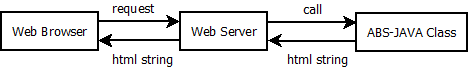
\includegraphics[
        width=0.8\textwidth
    ]{img/request-webserver-abs.png}
    \caption{Bagaimana web server menghasilkan sebuah halaman web}
    \label{fig:howAbsGenerateHTML}
\end{figure}

Untuk dapat mensimulasikan proses seperti yang telah digambarkan pada gambar \ref{fig:howAbsGenerateHTML} di atas, pertama-tama penulis membuat sebuah ABS Module yang fungsinya adalah untuk dapat menghasilkan sebuah halaman sederhana dan memberikannya kepada \textit{web server}. berikut adalah kode ABS yang penulis buat untuk menghasilkan sebuah halaman web:

\begin{lstlisting}[
caption=Kode ABS untuk menghasilkan halaman HTML,
label={lst:absWelcomeView},
]
module ABS.MVC.View.WelcomeView;

interface WelcomeView
{
	String generateView();
}

class WelcomeViewImpl implements WelcomeView
{
	
	String generateView() {		
		String html = "<!DOCTYPE HTML>";
		html = html + "<html>";
		html = html + "<body>";
		html = html + "<h1>Welcome!!</h1>";
		html = html + "Please login <a href='/login.abs'>here</a>";
		html = html + "<br />";
		html = html + "<p>This page was generated from ABS Class</p>";
		html = html + "</body>";
		html = html + "</html>";
		
		return html;
	}
}
\end{lstlisting}

Seperti yang terlihat pada kode \ref{lst:absWelcomeView} di atas, penulis menggunakan \texttt{String} berisikan kode HTML yang disambung-sambung (\textit{concatted String}) untuk menghasilkan sebuah halaman web. Rencananya adalah string yang sudah dihasilkan oleh halaman ABS Module ini nantinya akan diberikan ke \textit{web server} untuk kemudian diberikan ke \textit{web browser} dan ditampilkan ke \textit{user}. Sebagai awalan, penulis membuat sebuah class JAVA yang ditujukan untuk memanggil class JAVA hasil kompilasi ABS tersbeut untuk kemudian ditampilkan di \textit{console} dengan menggunakan \texttt{System.out.println()}. Berikut adalah kode JAVA yang dibuat oleh penulis beserta hasil pemanggilan class ABS-nya.

\begin{lstlisting}[
caption=Kode JAVA untuk memanggil ABS,
label={lst:javaCallABS},
escapeinside={@}{@}
]
package com.fmse.absserver;

public class ABSMain extends ABSObject 
{
    ...
       
    public ABSUnit run() {
        System.out.println("ABSMain running..");
        WelcomeView_i view = WelcomeViewImpl_c.__ABS_createNewObject(this); @\label{lst:javaCreateABSObject}@
        ABSString html = ABSRuntime.checkForNull(view).generateView(); @\label{lst:javaCallABSMethod}@
        System.out.println(html.getString());
        return ABSUnit.UNIT; 
    }
    
    public static void main(String[] args) throws Exception {
        StartUp.startup(new String[0], ABSMain.class);
    }
}
\end{lstlisting}

\begin{figure}
    \centering
    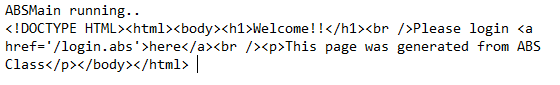
\includegraphics[
        width=0.8\textwidth
    ]{img/java-call-abs-result.png}
    \caption{Hasil dari pemanggilan ABS yang berisikan HTML String}
    \label{fig:javaABSCallResult}
\end{figure}

Terlihat pada kode \ref{lst:javaCallABS} baris \ref{lst:javaCreateABSObject} dan \ref{lst:javaCallABSMethod} di atas, penulis membuat sebuah \textit{instance} dari class \texttt{WelcomView} serta melakukan pemanggilan fungsi \texttt{generateView()} untuk mendapatkan \texttt{String} HTML yang telah dibuat. Hasil dari pemanggilan fungsi \texttt{generateView()} pada class \texttt{WelcomeView} tersebut adalah sebuah \texttt{String} panjang berisikan kode HTML seperti yang terlihat pada gambar \ref{fig:javaABSCallResult}.\\

Setelah penulis berhasil memanggil class JAVA hasil kompilasi ABS untuk mendapatkan HTML String, langkah selanjutnya adalah memberikan HTML String tersebut kepada web browser. Untuk dapat melakukan hal tersebut, penulis akan membuat sebuah web server sederhana dengan menggunakan class \texttt{ServerSocket} pada JAVA. Berikut adalah kode JAVA yang penulis buat untuk dapat menerima request dari \textit{web browser} dan memberikan halaman web yang diinginkan kepada \textit{web browser}.

\begin{lstlisting}[
caption=Potongan kode web server yang memanggil class ABS,
label={lst:javaSimpleWebServer},
escapeinside={@}{@}
]
public class ABSHttpServer extends ABSObject {

    ...
    
    public ABSUnit run() {
        try {
            ServerSocket serverSocket = new ServerSocket(8080); @\label{lst:javaCreateSocket}@
            while(true) {
                Socket remote = serverSocket.accept(); @\label{lst:javaCreateSocket2}@
                BufferedReader in = new BufferedReader(
                        new InputStreamReader(remote.getInputStream()));
                String request = in.readLine();
                String[] protocols = request.split(" ");
                
                ...
                
                if(protocols[1].equals("/")) { @\label{lst:serverStartCallABS}@
                	WelcomeView_i view = WelcomeViewImpl_c.__ABS_createNewObject(this); 
                    html = ABSRuntime.checkForNull(view).generateView().getString();
                    out.println(html);
                } @\label{lst:serverEndCallABS}@
                
                out.flush();
                remote.close();
            }
        }
        catch(Exception e) {
            e.printStackTrace();
        }
        
        return ABSUnit.UNIT;
    }
    
    ...
}
\end{lstlisting}

Pada kode \ref{lst:javaSimpleWebServer} baris \ref{lst:javaCreateSocket} dan \ref{lst:javaCreateSocket2} di atas, terlihat bahwa penulis melakukan pembuatan \texttt{ServerSocket} dan membuka \textit{port} 8080 untuk menerima \textit{request} dari \textit{web browser}. Setelah \textit{web server} menerima \textit{request} dari \textit{web browser}, berikutnya \textit{web server} akan mencocokan URL yang diberikan oleh \textit{web browser} seperti yang terlihat pada gambar \ref{fig:webBrowserRequest}. Apabila URL yang diminta cocok dengan salah satu kondisi yang ada di \textit{web server}, berikutnya \textit{web server} akan melakukan pemanggilan class ABS seperti yang terlihat pada kode \ref{lst:javaSimpleWebServer} baris \ref{lst:serverStartCallABS} - \ref{lst:serverEndCallABS}. Setelah HTML String berhasil diterima oleh \textit{web server} berikutnya akan diberikan ke \textit{web browser} melalui \texttt{OutputStream} pada \texttt{ServerSocket} untuk kemudian ditampilkan di \textit{web browser} seperti yang terlihat pada gambar di bawah ini.

\begin{figure}
    \centering
    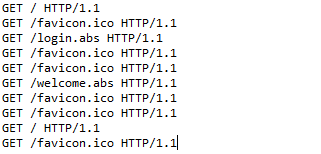
\includegraphics[
        width=0.6\textwidth
    ]{img/web-browser-request.png}
    \caption{Contoh \textit{request} dari \textit{web browser}}
    \label{fig:webBrowserRequest}
\end{figure}

\begin{figure}
    \centering
    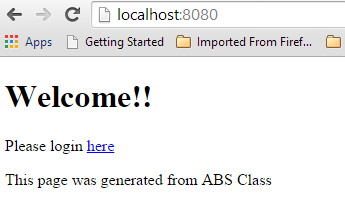
\includegraphics[
        width=0.6\textwidth
    ]{img/abs-welcome-view.png}
    \caption{Halaman web yang dibuat menggunakan ABS}
    \label{fig:javaABSCallResult}
\end{figure}

Sampai pada tahap ini penulis telah berhasil membuat sebuah halaman web sederhana dengan menggunakan ABS. Langkah berikutnya yang penulis lakukan adalah mencoba untuk memetakan ABS kedalam komponen-komponen MVC untuk membuat sebuah MVC Framework.

\section{Memetakan ABS kedalam komponen MVC}
Bagian ini menjelaskan tentang proses pemetaan ABS kedalam komponen Model, View dan Controller. Pada bagian ini juga akan dijelaskan tentang keputusan penulis dalam memilih thymeleaf templating engine sebagai pengganti ABS dalam membuat komponen View pada framework ABS MVC.

\section{Membuat Ant Script untuk mempermudah proses Compile dan Deployment}
Bagian ini menjelaskan tentang proses pembuatan ant script untuk mempermudah proses compile dan deployment dari yang sebelumnya menggunakan menu di eclipse menjadi ke terminal console.

\section{Menerima input POST dan GET dari web browser}
Bagian ini menjelaskan tentang eksperimen yang dilakukan oleh penulis dalam mencari tahu metode seperti apa yang dapat digunakan dalam menerima input HTTP POST dan GET dari web browser.

\section{Membuat Routing configuration}
Bagian ini menjelaskan tentang proses pembuatan routing configuration untuk memetakan setiap url kedalam class controller dan methodnya.
\chapter{Hasil Eksperimen}

%=============================
\section{ABS MVC Framework}
%=============================
ABS MVC Framework merupakan sebuah web application framework berbasis Model-View-Controller (MVC) yang dibangun dengan menggunakan bahasa pemodelan ABS. Tujuan dibangunnya framework ini adalah untuk membantu para pengembang perangkat lunak untuk memanfaatkan bahasa pemodelan ABS dalam menghasilkan sebuah perangkat lunak berbasis web. Selain itu, framework ini juga dapat membantu para pengembang perangkat lunak untuk dapat menerapkan pola MVC dalam proses pengembangan aplikasi web yang mereka buat. Penerapan pola MVC tersebut nantinya akan membantu para pengembang perangkat lunak dalam memisahkan logika aplikasi, data dan presentasi dari setiap baris kode yang dibuat sehingga akan meningkatkan \textit{maintainability} dari perangkat lunak yang dihasilkan.

\subsection{Arsitektur Framework}
Framework MVC ABS dibangun atas tiga bagian yang diantaranya adalah:
\begin{itemize}
    \item \textbf{HTTP Helper}: merupakan komponen framework yang bertugas untuk menangkap HTTP Request dan memberikan HTTP Response kepada web server. Komponen ini dibuat dengan menggunakan bahasa pemodelan ABS.
    \item \textbf{URL Router}: merupakan komponen framework yang bertugas untuk melakukan pemetaan terhadap setiap URL request yang diterima dari web server kedalam application Controller yang dibuat. komponen ini juga dibuat dengan menggunakan bahasa pemodelan ABS.
    \item \textbf{Application Builder}: merupakan komponen framework yang bertugas untuk melakukan proses kompilasi kode program dan membungkusnya kedalam bentuk JAVA Archive (jar) untuk kemudian di \textit{deploy} ke dalam web server. komponen ini dibuat dengan menggunakan Apache Ant.
\end{itemize}

\noindent
komponen-komponen framework di atas berperan dalam membantu para pengembang perangkat lunak untuk dapat menghasilkan sebuah perangkat lunak berbasis web dengan menggunakan bahasa pemodelan ABS.

\subsection{Struktur Direktori}
Struktur direkretori dalam sebuah framework MVC berperan dalam membantu para pengguna framework untuk mengatur peletakan setiap kode program yang mereka hasilkan sesuai dengan kategori / jenis dari kode program tersebut. Dengan adanya struktur direktori yang baik, akan membantu para pengembang perangkat lunak untuk dapat konsisten dalam meletakkan setiap kode program yang mereka hasilkan. berikut ini adalah struktur direktori dari framework MVC ABS:

\begin{itemize}
    \item \textbf{dist}: folder ini digunakan untuk menyimpan binary dari aplikasi web yang sudah di compile.
    \item \textbf{src}: folder ini digunakan untuk menyimpan file ABS yang dibuat oleh para pengembang perangkat lunak. folder ini memiliki sub folder "Model", "View" dan "Controller" yang digunakan untuk meletakkan komponen MVC yang dibuat.
    \item \textbf{lib}: folder ini berisi library yang dibutuhkan oleh framework MVC ABS untuk dapat meng-compile kode ABS dan mengubahnya ke dalam kode JAVA.
\end{itemize}

%=============================
\section{ABS MVC Server}
%=============================


\bibliography{conf/bib}
\bibliographystyle{conf/apalikerd}

\end{document}